\section{Histograms}


\begin{center}
	\begin{figure}[H]
		\subfloat[Raw data]{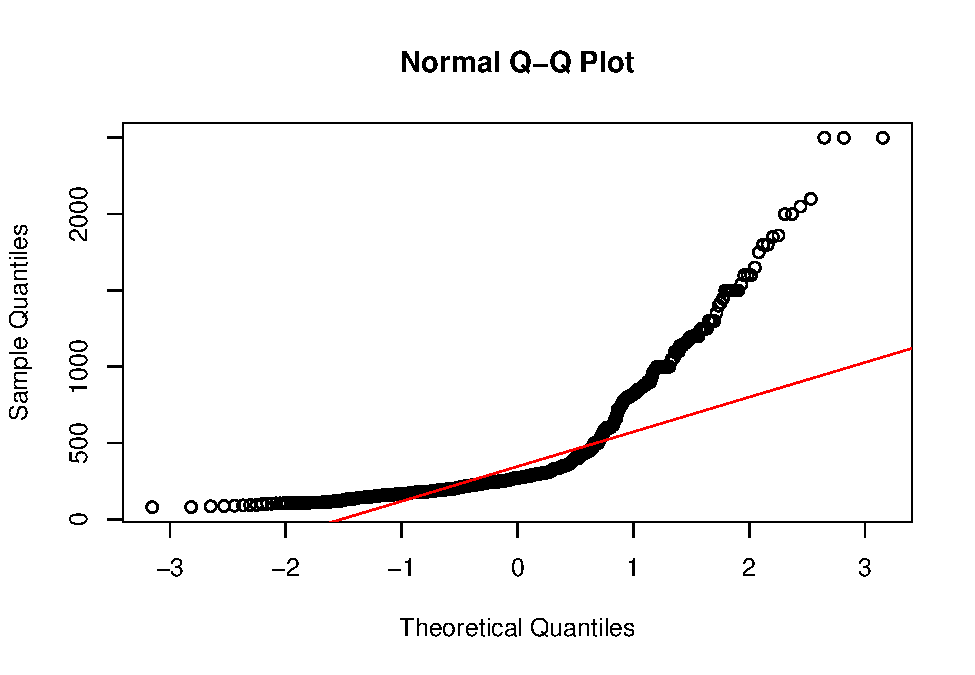
\includegraphics[scale=0.45]{MA_JJ_files/figure-latex/normalDistribution-1.pdf}}
		\subfloat[Logtransformed data]{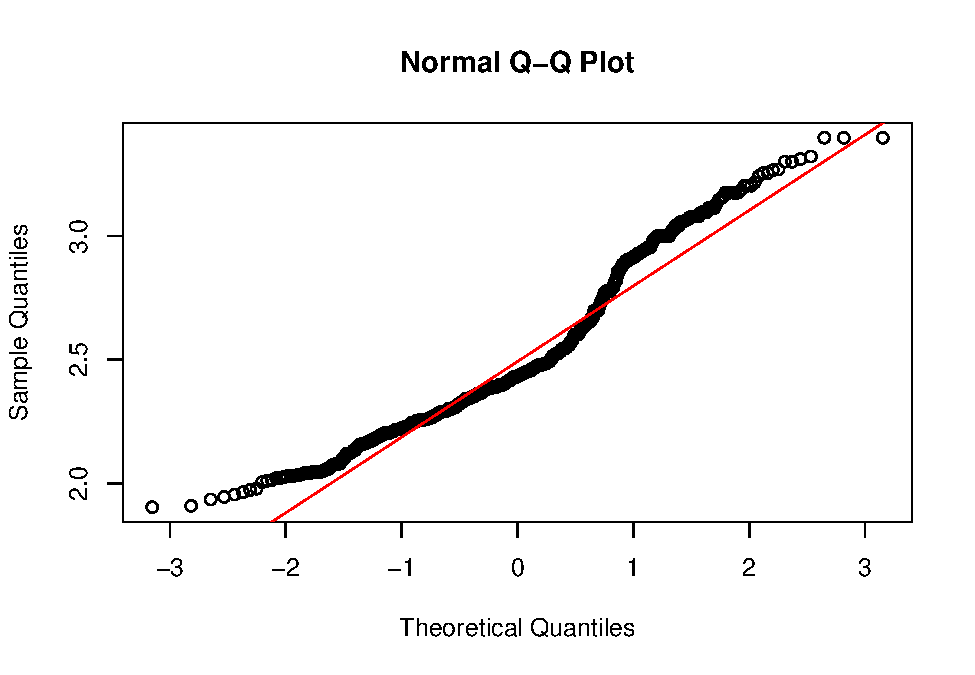
\includegraphics[scale=0.45]{MA_JJ_files/figure-latex/normalDistribution-2.pdf}}	
		\caption[Testing normal distribution]{Visual test for normal distribution. In case of normally distributed data, the black circles should follow the red line, which is not the case for either raw data nor logtransformed data. Therefore, data is not normally distributed.}
		\label{fig:NormDis}
	\end{figure}
\end{center}


\begin{center}
	\begin{figure}[H]
		\subfloat[Fossil vs. modern]{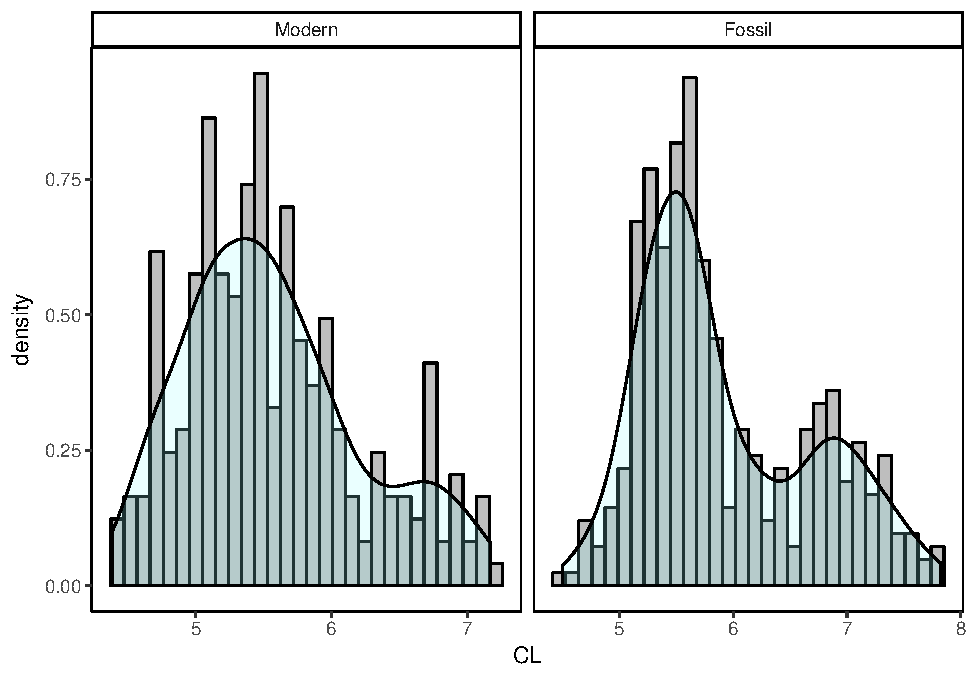
\includegraphics[scale=0.45]{MA_JJ_files/figure-latex/HistFosMo-1.pdf}}
		\subfloat[Continental vs. insular]{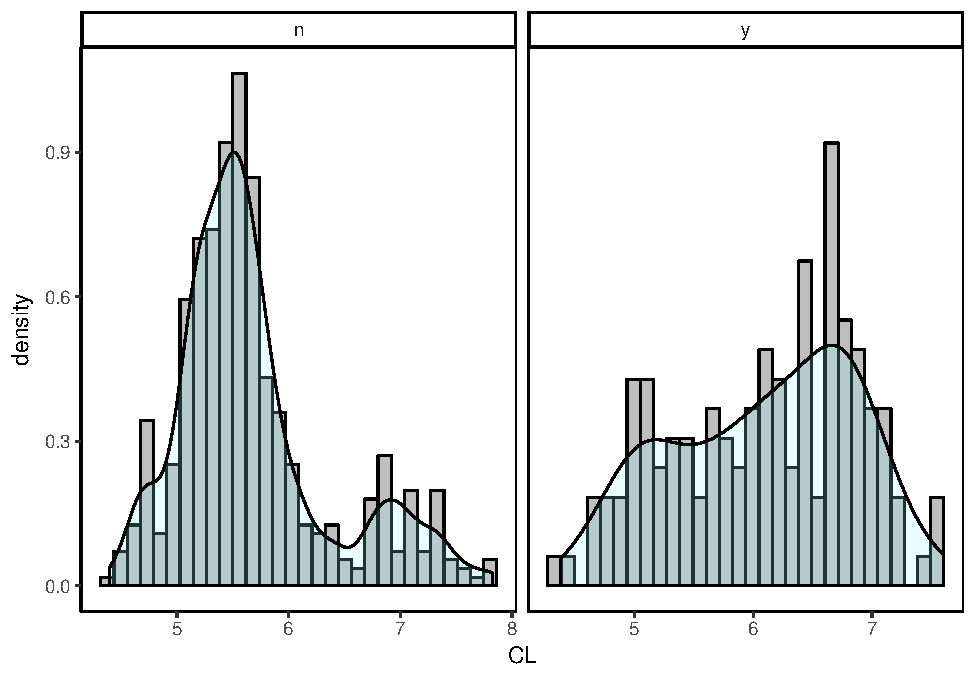
\includegraphics[scale=0.45]{MA_JJ_files/figure-latex/HistCI-1.pdf}}	
		\hfill %
		\subfloat[Fossil vs. modern, continental vs. insular]{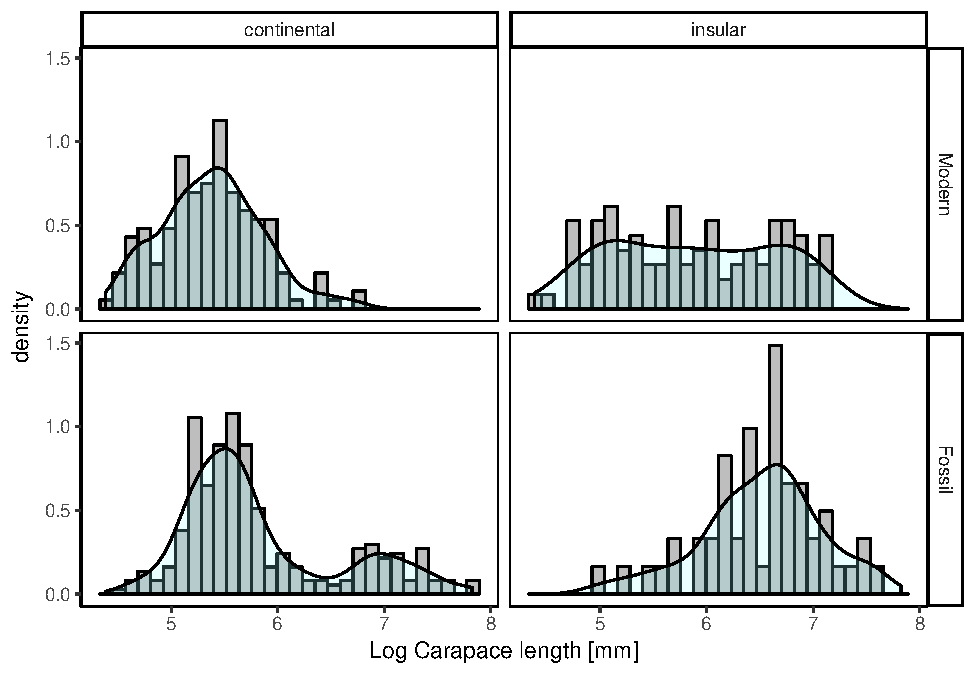
\includegraphics[scale=0.45]{MA_JJ_files/figure-latex/HistFMCI-1.pdf}}
		\subfloat[Per continent]{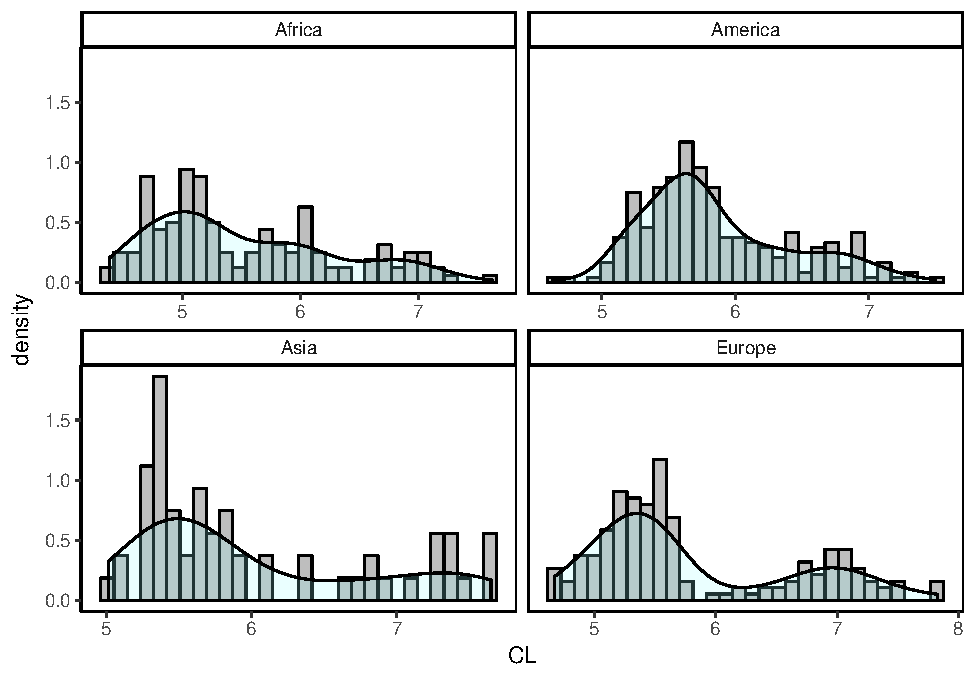
\includegraphics[scale=0.45]{MA_JJ_files/figure-latex/HistCon-1.pdf}}	
		\caption[Additional histograms]{Histograms for several subgroups of the dataset.}
		\label{fig:HistRest}
	\end{figure}
\end{center}